\documentclass[aspectratio=169]{beamer}
\usepackage{fontspec}
\usefonttheme{professionalfonts}
\usepackage{amsmath,amssymb,amsthm}
\usepackage{arydshln,mathtools}
\usepackage{bm}
\usepackage{color}
\definecolor{theme}{RGB}{0,73,114}
\usepackage{multicol}
%\usepackage[caption=false]{subfig}
\usepackage{subcaption}

\usepackage{comment}

\usepackage{graphicx}
\usepackage{diffcoeff}
\usepackage{dsfont}
\usepackage{mathrsfs}
\usepackage[most]{tcolorbox}

\usepackage{xspace}
\usepackage{appendixnumberbeamer}


\usepackage{media9}
\usepackage[backend=bibtex, style=verbose]{biblatex}

\bibliography{biblio_PH}
%\renewcommand\bibfont{\scriptsize}

\addtobeamertemplate{footnote}{\vspace{-6pt}\advance\hsize-0.5cm}{\vspace{6pt}}
\makeatletter
% Alternative A: footnote rule
\renewcommand*{\footnoterule}{\kern -3pt \hrule \@width 2in \kern 8.6pt}
% Alternative B: no footnote rule
% \renewcommand*{\footnoterule}{\kern 6pt}
\makeatother


\makeatletter
\g@addto@macro\normalsize{%
	\setlength\abovedisplayskip{5pt}
	\setlength\belowdisplayskip{5pt}
	\setlength\abovedisplayshortskip{5pt}
	\setlength\belowdisplayshortskip{5pt}
}
\makeatother

\graphicspath{{./imagesPH/}}



% Math macros
\DeclareMathOperator*{\grad}{grad}
\DeclareMathOperator*{\Grad}{Grad}
\DeclareMathOperator*{\Div}{Div}
\renewcommand{\div}{\operatorname{div}}
\DeclareMathOperator*{\Hess}{Hess}
\DeclareMathOperator*{\curl}{curl}


\DeclareMathOperator{\tr}{tr}

\DeclareMathOperator{\Dom}{Dom}
\DeclareMathOperator*{\esssup}{ess\,sup}

\newcommand{\bbR}{\mathbb{R}}
\newcommand{\bbI}{\mathbb{I}}
\newcommand{\bbC}{\mathbb{C}}
\newcommand{\bbF}{\mathbb{F}}
\newcommand{\bbA}{\mathbb{A}}
\newcommand{\bbB}{\mathbb{B}}
\newcommand{\bbS}{\mathbb{S}}


\newcommand{\inpr}[3][]{\ensuremath{( #2, \, #3 )_{#1}}}
\newcommand{\dualpr}[3][]{\ensuremath{\langle #2 \, \vert #3 \rangle_{#1}}}

\DeclareMathOperator*{\argmax}{arg\,max}
\DeclareMathOperator*{\argmin}{arg\,min}

\newtheorem{proposition}{Proposition}
\newtheorem{remark}{Remark}
\newtheorem{hypothesis}{Hypothesis}
\newtheorem{assumption}{Assumption}
\newtheorem{conjecture}{Conjecture}


\def\onedot{$\mathsurround0pt\ldotp$}
\def\cddot{% two dots stacked vertically
	\mathbin{\vcenter{\baselineskip.67ex
			\hbox{\onedot}\hbox{\onedot}}%
}}


\setbeamertemplate{blocks}[rounded][shadow]

\setbeamercolor{block body alerted}{bg=alerted text.fg!10}
\setbeamercolor{block title alerted}{bg=alerted text.fg!20}
\setbeamercolor{block body}{bg=structure!10}
\setbeamercolor{block title}{bg=structure!20}
\setbeamercolor{block body example}{bg=green!10}
\setbeamercolor{block title example}{bg=green!20}

% Remove navigation bar
\setbeamertemplate{navigation symbols}{}

\addtobeamertemplate{navigation symbols}{}{%
	\usebeamerfont{footline}%
	\usebeamercolor[fg]{footline}%
	\hspace{1em}%
	\insertframenumber/\inserttotalframenumber
}


\makeatletter \renewcommand\d[1]{\ensuremath{%
		\;\mathrm{d}#1\@ifnextchar\d{\!}{}}}
\makeatother


\newif\iftocsub
\tocsubtrue
\AtBeginSection[] {
	\begin{frame}[noframenumbering]{Outline}
		\tableofcontents[sectionstyle=show/shaded, subsectionstyle=show/show/hide]
	\end{frame}
	\tocsubfalse
}
\AtBeginSubsection[] {
	\iftocsub
	\begin{frame}[noframenumbering]{Outline}
		\tableofcontents[currentsubsection, sectionstyle=show/shaded, subsectionstyle=show/shaded/hide]
	\end{frame}
	\fi
	\tocsubtrue
}

\newcommand{\beginbackup}{
	\newcounter{framenumbervorappendix}
	\setcounter{framenumbervorappendix}{\value{framenumber}}
}
\newcommand{\backupend}{
	\addtocounter{framenumbervorappendix}{-\value{framenumber}}
	\addtocounter{framenumber}{\value{framenumbervorappendix}} 
}


\begin{document}
	
	
	\begin{frame}[plain]
		
		%%%%%%%% Title slide details %%%%%%%%%%%%%%


% Background Image
\newcommand{\myBackground}
{
    
\includegraphics[height=1.02\paperheight,page=9]{beamerthemeutresources}
}

% Title
\newcommand{\myTitle}
{
Improving multiphysics simulation through port-Hamiltonian system theory
}

% Subtitle
\newcommand{\mySubTitle}
{
}

% Author
\newcommand{\myAuthor}   
{
    Andrea Brugnoli
}

% Affiliation
\newcommand{\myAffiliate}
{
  
}

% Presentation Date
\newcommand{\myDate}   
{
    28 June 2022
}

% Logo
\newcommand{\myLogo}   
{
    
\includegraphics[width=3cm]{Logo.png}
}
%%%%%%%%%%%%%%%%%%%%%%%%%%%%%%%%%%%%


%%%%%%%%%% Title slide code %%%%%%%%%%%
\begin{tikzpicture}[remember picture,overlay]

% Background color

\fill[white] (current page.south west) rectangle (current page.north east);
% Background image
\node[above right,inner sep=0pt] at (current page.south west)
    {
        \myBackground
    };
    
% Title & Subtitle
\node
[
    above=0.5cm,
    align=center,
    draw=black!50,
    % rounded corners,
    double,
    double distance=0.1cm,
    double=blue!10,
    fill=theme!10,
    inner xsep=15pt,
    inner ysep=10pt, 
    minimum width=0.8\textwidth,
    text width=0.8\textwidth
] (title) at (current page.center)
{
    \LARGE \myTitle  \\[5pt]
    \small \mySubTitle
};

% Author 
\node[ below=0.5cm] (author) at (title.south){\myAuthor};

% Author 
\node[ below=0.25cm ](affiliate) at (author.south){\small \myAffiliate};

% Date
\node[below=0.25] (date) at (affiliate.south){\large \myDate};

% Logo
\node
[
    below =0.25cm
] at (date.south)
{
    \myLogo
};

\end{tikzpicture}
		
	\end{frame}
	
	
	\begin{frame}{Outline}
		
		\tableofcontents
		
	\end{frame}

\section{Multiphysics problems}


\begin{frame}{Challenges in muliphysics problems}
	
	Multiphysics problems are commomly found in industrial applications.
	\begin{figure}[t]
		\begin{subfigure}[t]{0.34\textwidth}
			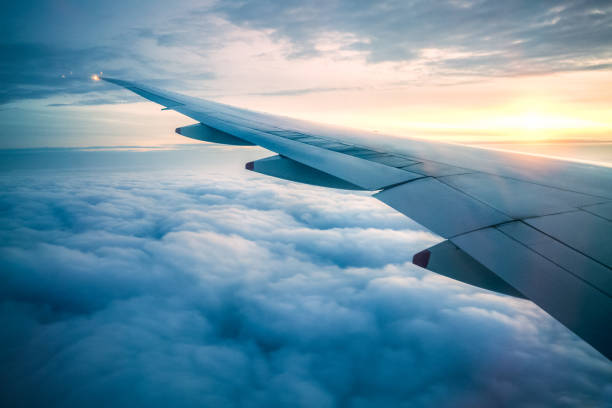
\includegraphics[width=\columnwidth]{wing.jpg}\\
			\centering{Aeroelasticity}%
		\end{subfigure}\hfill
		\begin{subfigure}[t]{0.3\textwidth}
			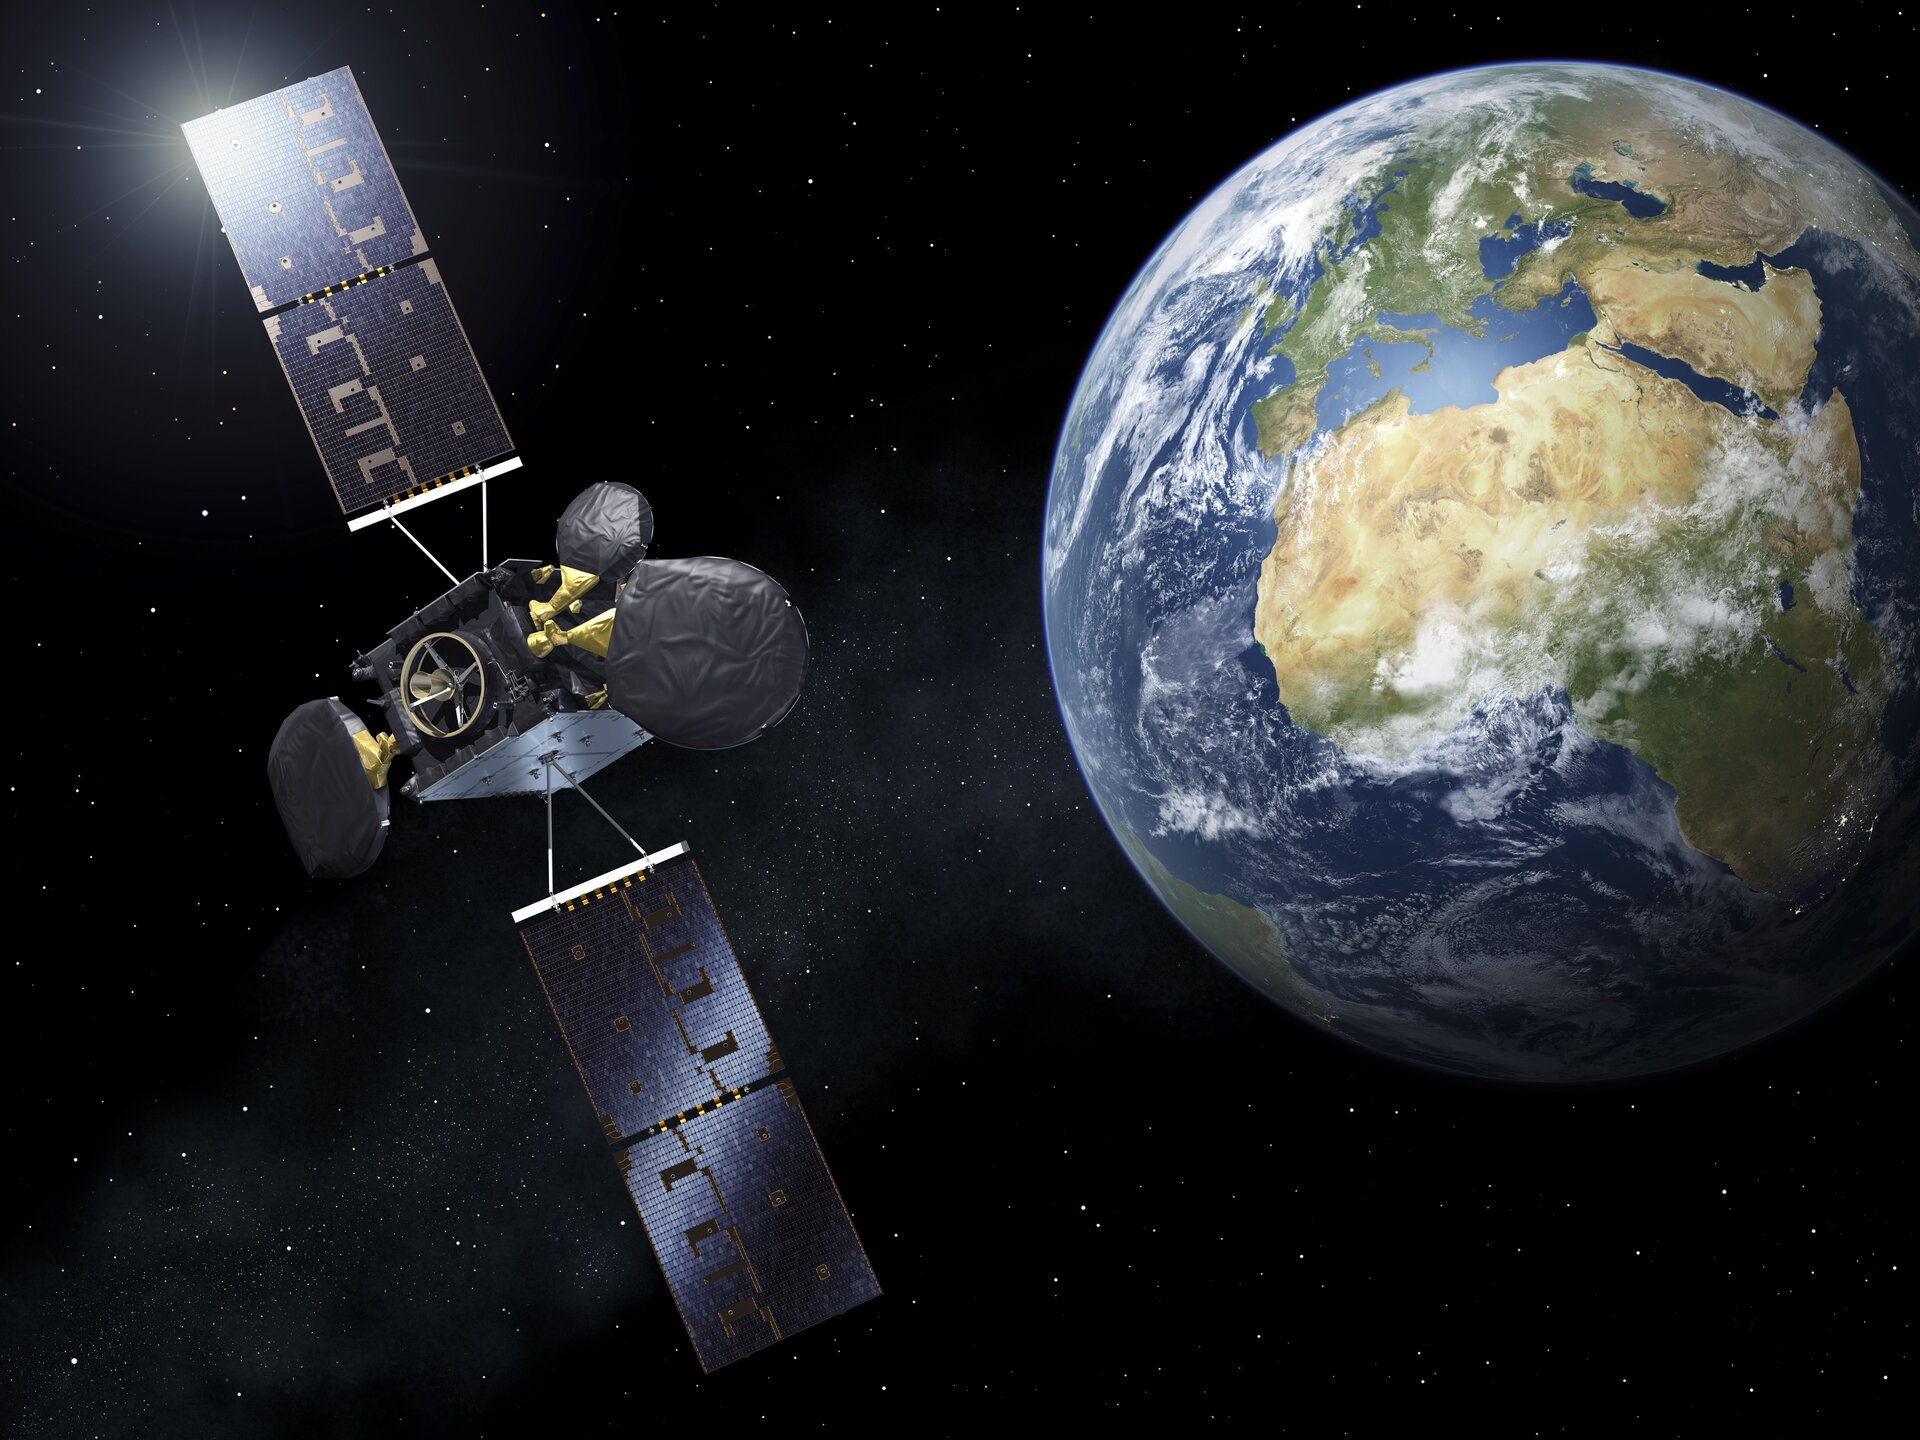
\includegraphics[width=\columnwidth]{esa_satellite.jpg}\\
			\centering{Thermoelasticity} 
		\end{subfigure}\hfill
		\begin{subfigure}[t]{0.26\textwidth}
			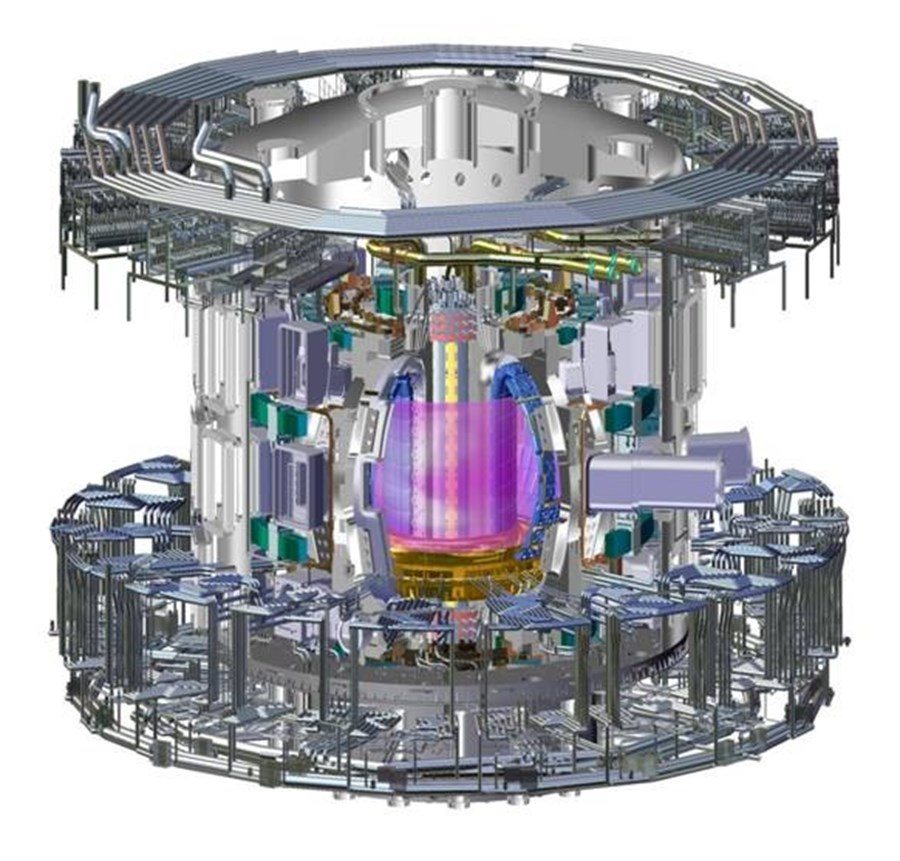
\includegraphics[width=\columnwidth]{tcws.jpg}\\
			\centering{Magnetohydrodynamics}
		\end{subfigure}
	\end{figure}
	Challenges:
	\begin{itemize}
		\item Coupling between different models.​
		\item Huge computational cost due to the large size of the models.​
		\item Multidisciplinary optimization for dynamical systems.​
	\end{itemize}
	
\end{frame}


\begin{frame}{Typical workflow in industry}
	
	\begin{itemize}
		\item Specific modelling and numerical methods for each physical domain. 
			\begin{itemize}
			\item[\textcolor{red}{$\times$}] The open character of systems is not properly considered.
			\item[\textcolor{red}{$\times$}] Numerical methods do not preserve the structure required to interconnect systems.
		\end{itemize}
		\item Model reduction via statistical methods.
	\begin{itemize}
		\item[\textcolor{red}{$\times$}] The physical structure of the model is lost and first principles are violated.
		\item[\textcolor{red}{$\times$}] This methodology does not generalize to different problems.
	\end{itemize}
\vspace{.3cm}
	\begin{figure}[t]
		\centering
		\begin{subfigure}[t]{0.4\textwidth}
			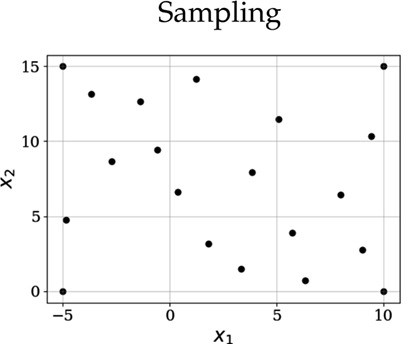
\includegraphics[width=.8\columnwidth]{sampling.jpg}
		\end{subfigure}\hspace{1cm}
		\begin{subfigure}[t]{0.4\textwidth}
			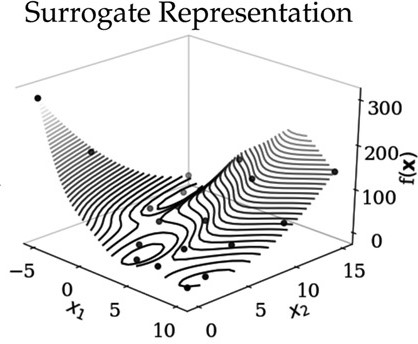
\includegraphics[width=.8\columnwidth]{surrogate_model.jpg}
		\end{subfigure}
	\end{figure}
	\end{itemize}
\end{frame}

\begin{frame}{Example: convection dominated transport}
	Convection dominated transport of a passive scalar field in a Stokes flow\footcite{volker2017review}
	\begin{equation*}
		\begin{aligned}
			\nu \Delta \bm{u} + \nabla p &=0, \\
			\nabla \cdot \bm{u} &=0, \\
			-\varepsilon \Delta \theta + \bm{u} \cdot \nabla \theta &=0.
		\end{aligned} \qquad \qquad 
	\begin{aligned}
		\bm{u} &: \text{Velocity}, \\
		p &: \text{Pressure}, \\
		\theta &: \text{Temperature}.
	\end{aligned}
	\end{equation*}
	\begin{figure}
		\centering
		\includegraphics[width=.75\textwidth]{channel_convection_T.eps}
		\caption*{Geometry and boundary conditions}
	\end{figure}
\end{frame}

\begin{frame}{When multiphysics goes wrong}
	Exact solution for the temperature $\theta_{\mathrm{ex}}= 1$.
	\begin{itemize}
		\item $(\bm{u}, p)$ discretized using the Taylor-Hood element $\mathbb{P}_2/\mathbb{P}_1$;
		\item $\theta$ discretized via Voronoi finite volume method.
	\end{itemize}
The Taylor-Hood element does not lead to divergence free velocity $||\nabla \cdot \bm{u}||_{L^2(\Omega)} \neq 0$.
\begin{figure}[t]
	\begin{subfigure}[t]{0.32\textwidth}
		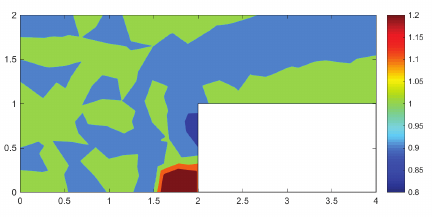
\includegraphics[width=\columnwidth]{Concentration_ref1.png}\\
		\centering{Refinement 1}%
	\end{subfigure}\hfill
	\begin{subfigure}[t]{0.32\textwidth}
		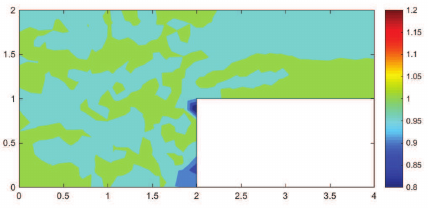
\includegraphics[width=\columnwidth]{Concentration_ref2.png}\\
		\centering{Refinement 2} 
	\end{subfigure}\hfill
	\begin{subfigure}[t]{0.32\textwidth}
		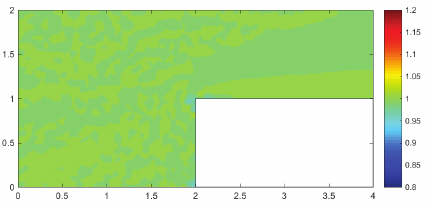
\includegraphics[width=\columnwidth]{Concentration_ref3.png}\\
		\centering{Refinement 3}
	\end{subfigure}
\caption{Discrete temperature field $\theta$ obtained }
\end{figure}

\end{frame}

\section{Port-Hamiltonian systems as a unified language for multiphysics}

\begin{frame}{A unified language for multiphysics in engineering}
	The port-Hamiltonian paradigm provides a language to understand multiphysics:
	\vspace{.5cm}
	\begin{columns}
		\begin{column}{.6\textwidth}
			\begin{itemize}
				\item The idea of \textbf{interconnection} is formalized as \textbf{duality pairing}.
				\item \textbf{Physics} is at the core: port-Hamiltonian systems are \textbf{passive} with respect to the \textbf{energy storage function}.
				\item The \textbf{topological} and \textbf{metrical} structure of the equation is clearly separated (mimetic discretization).
			\end{itemize}
		\end{column}
		\begin{column}{.4\textwidth}
			\centering
			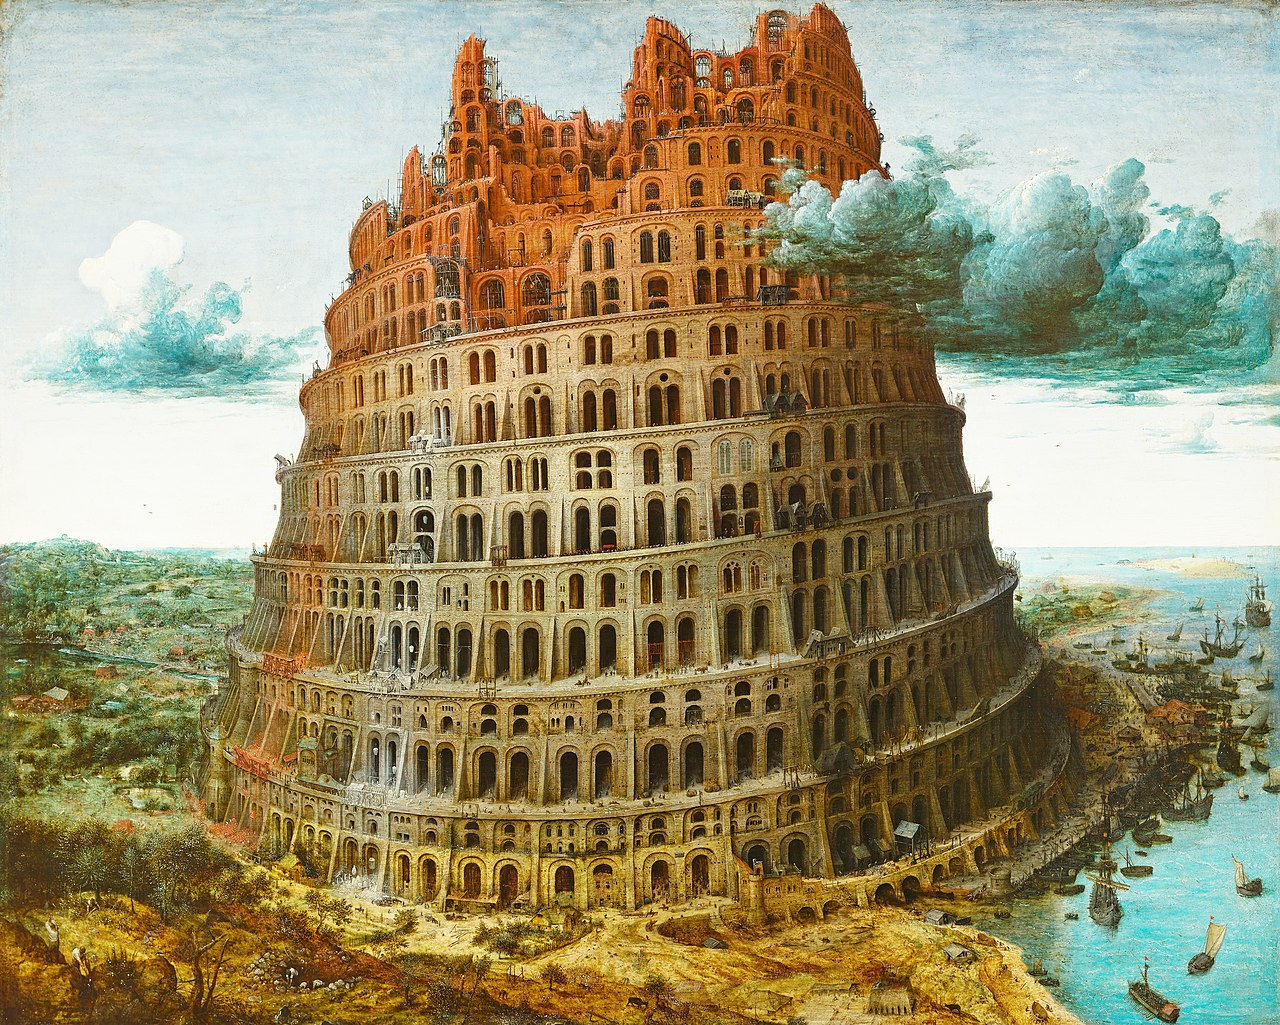
\includegraphics[width=.9\columnwidth]{babel_tower.jpeg}
		\end{column}
	\end{columns}

\end{frame}

\subsection{Functional analytic structure}

\begin{frame}{A simple definition\footcite{reis2021pH}}
	\begin{definition}[Port-Hamiltonian system]
		Let $X_\mathcal{S}, \; X_\mathcal{R}, \; \mathcal{X}_S$ be Banach spaces. A port-Hamiltonian system is a triple $(\mathcal{D}, H, \mathcal{R})$:
		\begin{itemize}
			\item $\mathcal{D} \subset (X_\mathcal{S}, \; X_\mathcal{R}, \; X_\mathcal{P}) \times (X^{'}_\mathcal{S}, \; X^{'}_\mathcal{R}, \; X^{'}_\mathcal{P})$ is a Dirac structure.
			\item $\mathcal{H} : U \rightarrow \bbR$ (with $U \subset X_\mathcal{S}$ open) is a Hamiltonian.
			\item $\mathcal{R}\subset X_\mathcal{R} \times X_{\mathcal{R}}^{'}$ is a resistive relation.
		\end{itemize}
		The behavior of the pH system on an interval $\mathbb{I} \subset \bbR$ consists of all $(x, f_{\mathcal{R}}, f_{\mathcal{P}} , e_{\mathcal{R}}, e_{\mathcal{P}})$
		\begin{itemize}
			\item 	$x \in W^{1,2}_{\text{loc}}(\mathbb{I}, X_{\mathcal{S}})$, and $x(t) \in U, \; \forall t \in \bbI$, 
			\item $(f_\mathcal{R}, e_\mathcal{R}) \in L^2_{\text{loc}}(\bbI; X_{\mathcal{R}} \times X^{'}_{\mathcal{R}})$ and $(f_\mathcal{P}, e_\mathcal{P}) \in L^2_{\text{loc}}(\bbI; X_{\mathcal{P}} \times X^{'}_{\mathcal{P}})$
		\end{itemize}
		that fulfill the differential inclusion
		\begin{equation*}
			(-\diff{x}{t},\, f_{\mathcal{R}},\, f_{\mathcal{P}},\, D\mathcal{H}(x(t)),\, e_{\mathcal{R}},\, e_{\mathcal{P}}) \in \mathcal{D}, \qquad (f_\mathcal{R}, e_\mathcal{R}) \in \mathcal{R}, \qquad \text{for almost all } t \in \bbI.
		\end{equation*}
	\end{definition}
\end{frame}

\begin{frame}{Some mathematical definitions}
	\begin{block}{Dirac structure}
			Let $X$ be a Banach space. A subspace $\mathcal{D}\subset X \times X^{'}$ is called a Dirac structure, if $\forall \, f \in X, e \in X^{'}$, it holds
			\begin{equation*}
				(f, e) \in \mathcal{D} \iff \left( \dualpr{f}{\hat{e}} + \dualpr{\hat{f}}{e}=0, \quad \forall\, (\hat{f}, \hat{e})\right).
			\end{equation*}
		\end{block}

		\begin{block}{Hamiltonian}
			Let $X$ be a Banach space and $U \subset X$ be open. A mapping $\mathcal{H} : U \rightarrow \bbR$ is a Hamiltonian if it is locally Lipschitz continuous and G\^{a}teaux differentiable
		\end{block}
		
		\begin{block}{Resistive relation}
			Let $X$ be a Banach space.
			A relation $\mathcal{R} \subset X \times X^{'}$ is called resistive, if
			\begin{equation*}
				\dualpr{f}{e} \le 0, \qquad \forall\, (f,e) \in \mathcal{R}.
			\end{equation*}
		
		\end{block}

\end{frame}

\begin{frame}{Operators}
	If $J \in \mathcal{L}(X^{'}, X)$ is a skew-dual operator $\dualpr{J v}{w}= \dualpr{v}{-Jw}\; \forall\, v, w \in X^{'}$ then $D = \{(J e, e) : e \in X^{'}\}$ is a Dirac structure\footcite{reis2022passivity}.\\
	\vspace{.2cm}
	If $R :X^{'} \rightarrow X$ is dissipative $\dualpr{x{'}}{G(x{'})} \le 0,\; \forall \, x{'} \in X^{'}$, then $\mathcal{R} = \{(G(e), e) : e \in X^{'}\}$ is a resistive relation.
	
	\begin{equation*}
		\begin{pmatrix}
			\partial_t x \\
			f_\mathcal{R} \\
			f_\mathcal{P} \\
		\end{pmatrix} =
		J
		\begin{pmatrix}
			D\mathcal{H}(x(t)) \\
			e_\mathcal{R} \\
			e_\mathcal{P} \\
		\end{pmatrix}, \qquad f_{\mathcal{R}} = G(e_{\mathcal{R}}).
	\end{equation*}
\end{frame}

\begin{frame}{Example: the wave equation}
	Consider the Hamiltonian
	\begin{equation*}
		\mathcal{H} = \inpr[L^2(\Omega)]{p}{\kappa p} + \inpr[L^2(\Omega, \bbR^3)]{\bm{u}}{\rho^{-1}\bm{u}}.
	\end{equation*}
	where $\kappa$ is the Bulk modulus and $\rho$ is the density. \\
	\vspace{.5cm}
	The wave equation on $\Omega \subset \bbR^3$ with Dirichlet boundary condition reads:
	\begin{equation*}
			\begin{pmatrix}
			\partial_t p \\
			\partial_{t} \bm{u} \\
		\end{pmatrix} =
		\begin{bmatrix}
			0 & \div \\
			\grad_w & 0
		\end{bmatrix}
		\begin{pmatrix}
			D\mathcal{H}(p(t)) \\
			D\mathcal{H}(\bm{u}(t)) \\
		\end{pmatrix}, \qquad D\mathcal{H}(p(t))|_{\partial\Omega} = g. 
	\end{equation*}
where $\grad_w$ corresponds to a weak definition of the gradient.\\
In this case: $X_{\mathcal{S}}= L^2(\Omega) \times H^{\div}(\Omega)^{'}, \; X_{\mathcal{R}} = \emptyset, \; X_{\mathcal{P}}= H^{1/2}(\Omega)$ and
\begin{equation*}
		J = \begin{bmatrix}
			0 & \div & \gamma_0 \\
			\grad_w & 0 & 0 \\
			\gamma_{\bm{n}} & 0 & 0 
		\end{bmatrix}
	\end{equation*}
where $\gamma_0$ is the Dirichlet trace  and $\gamma_{\bm{n}}$ is the normal trace.

\end{frame}

\begin{frame}{Example: the Maxwell equations}
	Consider the Hamiltonian:
	\begin{equation*}
		\mathcal{H} = \frac{1}{2} \inpr[L^2(\Omega, \bbR^3)]{\bm{D}}{\varepsilon^{-1}\bm{D}} + \frac{1}{2} \inpr[L^2(\Omega, \bbR^3)]{\bm{B}}{\mu^{-1}\bm{B}}.
	\end{equation*}
where  $\varepsilon$ is the electric permittivity and $\mu$ is the magnetic permeability.\\
\vspace{.5cm}
	The Maxwell equation on $\Omega \subset \bbR^3$ with conducting boundary condition reads:
	\begin{equation*}
		\diffp{}{t}\begin{pmatrix}
			\bm{D} \\ \bm{B} 
		\end{pmatrix} = 
		\begin{bmatrix}
			0 & \curl \\
			-\curl_w & 0 \\
		\end{bmatrix}
		\begin{pmatrix}
			D\mathcal{H}(\bm{D}(t)) \\
			D\mathcal{H}(\bm{B}(t)) \\
		\end{pmatrix},\qquad D\mathcal{H}(\bm{D}(t)) \times \bm{n}|_{\partial\Omega}=0,
	\end{equation*}
	where $\curl_w$ corresponds to a weak $\curl$ operator and the field $\bm{D}, \; \bm{B}$ satisfy
	\begin{equation*}
			\nabla \cdot \bm{D}= 0, \qquad	\nabla \cdot \bm{B}= 0.
	\end{equation*}
In this case: $X_{\mathcal{S}}= L^2(\Omega, \bbR^3|\div=0) \times H^{\curl}(\Omega| \div=0)^{'}, \; X_{\mathcal{R}} = \emptyset, \; X_{\mathcal{P}}= \emptyset$ and
\begin{equation*}
	J = \begin{bmatrix}
		0 & \curl \\
		\curl_w & 0 \\
	\end{bmatrix}.
\end{equation*}


	
	
\end{frame}

\begin{frame}{And many more}
	The same framework applies to
	\begin{itemize}
		\item Linear and non-linear solid mechanics (beams, plates, shells, etc.).\\
		\item Fluid dynamics. \\
		\item Chemical reactions.
	\end{itemize}
\end{frame}



\subsection{The geometric definition}


\begin{frame}{The canonical geometric port-Hamiltonian system}
	Distributed port-Hamiltonian were initially defined in a differential geometric setting\footcite{vanderSchaft2002}.\\
	
	Given two fields  of smooth differential forms $\alpha^p \in \Lambda^p(\Omega)$ and $\beta \in \Lambda^q(\Omega)$ the following systems
	\begin{equation*}
		\begin{pmatrix}
			\partial_t \alpha^p \\
			\partial_t \beta^q\\
		\end{pmatrix} = 
		-\begin{bmatrix}
			0 & (-1)^r\d \\
			\d & 0 \\
		\end{bmatrix}
		\begin{pmatrix}
			\delta_{\alpha} H^{n-p}\\
			\delta_{\beta} H^{n-q}\\
		\end{pmatrix}
	\end{equation*}


\end{frame}


\section{Mimetic discretization of port-Hamiltonian systems}
	
\begin{frame}{Bibliography}
	%\bibliographystyle{unsrt}
	\nocite{*}
	\printbibliography
\end{frame}

	\appendix
	
	
	
	
\end{document}